\documentclass[a4paper]{article}

\def\ntitle{Markov Chains}
\def\ndate{Michaelmas, 2017 -- 2018}

\ifx \nauthor\undefined
  \def\nauthor{Qiangru Kuang}
\else
\fi

\ifx \ntitle\undefined
  \def\ntitle{Template}
\else
\fi

\ifx \nauthoremail\undefined
  \def\nauthoremail{qk206@cam.ac.uk}
\else
\fi

\ifx \ndate\undefined
  \def\ndate{\today}
\else
\fi

\title{\ntitle}
\author{\nauthor}
\date{\ndate}

%\usepackage{microtype}
\usepackage{mathtools}
\usepackage{amsthm}
\usepackage{stmaryrd}%symbols used so far: \mapsfrom
\usepackage{empheq}
\usepackage{amssymb}
\let\mathbbalt\mathbb
\let\pitchforkold\pitchfork
\usepackage{unicode-math}
\let\mathbb\mathbbalt%reset to original \mathbb
\let\pitchfork\pitchforkold

\usepackage{imakeidx}
\makeindex[intoc]

%to address the problem that Latin modern doesn't have unicode support for setminus
%https://tex.stackexchange.com/a/55205/26707
\AtBeginDocument{\renewcommand*{\setminus}{\mathbin{\backslash}}}
\AtBeginDocument{\renewcommand*{\models}{\vDash}}%for \vDash is same size as \vdash but orginal \models is larger
\AtBeginDocument{\let\Re\relax}
\AtBeginDocument{\let\Im\relax}
\AtBeginDocument{\DeclareMathOperator{\Re}{Re}}
\AtBeginDocument{\DeclareMathOperator{\Im}{Im}}
\AtBeginDocument{\let\div\relax}
\AtBeginDocument{\DeclareMathOperator{\div}{div}}

\usepackage{tikz}
\usetikzlibrary{automata,positioning}
\usepackage{pgfplots}
%some preset styles
\pgfplotsset{compat=1.15}
\pgfplotsset{centre/.append style={axis x line=middle, axis y line=middle, xlabel={$x$}, ylabel={$y$}, axis equal}}
\usepackage{tikz-cd}
\usepackage{graphicx}
\usepackage{newunicodechar}

\usepackage{fancyhdr}

\fancypagestyle{mypagestyle}{
    \fancyhf{}
    \lhead{\emph{\nouppercase{\leftmark}}}
    \rhead{}
    \cfoot{\thepage}
}
\pagestyle{mypagestyle}

\usepackage{titlesec}
\newcommand{\sectionbreak}{\clearpage} % clear page after each section
\usepackage[perpage]{footmisc}
\usepackage{blindtext}

%\reallywidehat
%https://tex.stackexchange.com/a/101136/26707
\usepackage{scalerel,stackengine}
\stackMath
\newcommand\reallywidehat[1]{%
\savestack{\tmpbox}{\stretchto{%
  \scaleto{%
    \scalerel*[\widthof{\ensuremath{#1}}]{\kern-.6pt\bigwedge\kern-.6pt}%
    {\rule[-\textheight/2]{1ex}{\textheight}}%WIDTH-LIMITED BIG WEDGE
  }{\textheight}% 
}{0.5ex}}%
\stackon[1pt]{#1}{\tmpbox}%
}

%\usepackage{braket}
\usepackage{thmtools}%restate theorem
\usepackage{hyperref}

% https://en.wikibooks.org/wiki/LaTeX/Hyperlinks
\hypersetup{
    %bookmarks=true,
    unicode=true,
    pdftitle={\ntitle},
    pdfauthor={\nauthor},
    pdfsubject={Mathematics},
    pdfcreator={\nauthor},
    pdfproducer={\nauthor},
    pdfkeywords={math maths \ntitle},
    colorlinks=true,
    linkcolor={red!50!black},
    citecolor={blue!50!black},
    urlcolor={blue!80!black}
}

\usepackage{cleveref}



% TODO: mdframed often gives bad breaks that cause empty lines. Would like to switch to tcolorbox.
% The current workaround is to set innerbottommargin=0pt.

%\usepackage[theorems]{tcolorbox}





\usepackage[framemethod=tikz]{mdframed}
\mdfdefinestyle{leftbar}{
  %nobreak=true, %dirty hack
  linewidth=1.5pt,
  linecolor=gray,
  hidealllines=true,
  leftline=true,
  leftmargin=0pt,
  innerleftmargin=5pt,
  innerrightmargin=10pt,
  innertopmargin=-5pt,
  % innerbottommargin=5pt, % original
  innerbottommargin=0pt, % temporary hack 
}
%\newmdtheoremenv[style=leftbar]{theorem}{Theorem}[section]
%\newmdtheoremenv[style=leftbar]{proposition}[theorem]{proposition}
%\newmdtheoremenv[style=leftbar]{lemma}[theorem]{Lemma}
%\newmdtheoremenv[style=leftbar]{corollary}[theorem]{corollary}

\newtheorem{theorem}{Theorem}[section]
\newtheorem{proposition}[theorem]{Proposition}
\newtheorem{lemma}[theorem]{Lemma}
\newtheorem{corollary}[theorem]{Corollary}
\newtheorem{axiom}[theorem]{Axiom}
\newtheorem*{axiom*}{Axiom}

\surroundwithmdframed[style=leftbar]{theorem}
\surroundwithmdframed[style=leftbar]{proposition}
\surroundwithmdframed[style=leftbar]{lemma}
\surroundwithmdframed[style=leftbar]{corollary}
\surroundwithmdframed[style=leftbar]{axiom}
\surroundwithmdframed[style=leftbar]{axiom*}

\theoremstyle{definition}

\newtheorem*{definition}{Definition}
\surroundwithmdframed[style=leftbar]{definition}

\newtheorem*{slogan}{Slogan}
\newtheorem*{eg}{Example}
\newtheorem*{ex}{Exercise}
\newtheorem*{remark}{Remark}
\newtheorem*{notation}{Notation}
\newtheorem*{convention}{Convention}
\newtheorem*{assumption}{Assumption}
\newtheorem*{question}{Question}
\newtheorem*{answer}{Answer}
\newtheorem*{note}{Note}
\newtheorem*{application}{Application}

%operator macros

%basic
\DeclareMathOperator{\lcm}{lcm}

%matrix
\DeclareMathOperator{\tr}{tr}
\DeclareMathOperator{\Tr}{Tr}
\DeclareMathOperator{\adj}{adj}

%algebra
\DeclareMathOperator{\Hom}{Hom}
\DeclareMathOperator{\End}{End}
\DeclareMathOperator{\id}{id}
\DeclareMathOperator{\im}{im}
\DeclarePairedDelimiter{\generation}{\langle}{\rangle}

%groups
\DeclareMathOperator{\sym}{Sym}
\DeclareMathOperator{\sgn}{sgn}
\DeclareMathOperator{\inn}{Inn}
\DeclareMathOperator{\aut}{Aut}
\DeclareMathOperator{\GL}{GL}
\DeclareMathOperator{\SL}{SL}
\DeclareMathOperator{\PGL}{PGL}
\DeclareMathOperator{\PSL}{PSL}
\DeclareMathOperator{\SU}{SU}
\DeclareMathOperator{\UU}{U}
\DeclareMathOperator{\SO}{SO}
\DeclareMathOperator{\OO}{O}
\DeclareMathOperator{\PSU}{PSU}

%hyperbolic
\DeclareMathOperator{\sech}{sech}

%field, galois heory
\DeclareMathOperator{\ch}{ch}
\DeclareMathOperator{\gal}{Gal}
\DeclareMathOperator{\emb}{Emb}



%ceiling and floor
%https://tex.stackexchange.com/a/118217/26707
\DeclarePairedDelimiter\ceil{\lceil}{\rceil}
\DeclarePairedDelimiter\floor{\lfloor}{\rfloor}


\DeclarePairedDelimiter{\innerproduct}{\langle}{\rangle}

%\DeclarePairedDelimiterX{\norm}[1]{\lVert}{\rVert}{#1}
\DeclarePairedDelimiter{\norm}{\lVert}{\rVert}



%Dirac notation
%TODO: rewrite for variable number of arguments
\DeclarePairedDelimiterX{\braket}[2]{\langle}{\rangle}{#1 \delimsize\vert #2}
\DeclarePairedDelimiterX{\braketthree}[3]{\langle}{\rangle}{#1 \delimsize\vert #2 \delimsize\vert #3}

\DeclarePairedDelimiter{\bra}{\langle}{\rvert}
\DeclarePairedDelimiter{\ket}{\lvert}{\rangle}




%macros

%general

%divide, not divide
\newcommand*{\divides}{\mid}
\newcommand*{\ndivides}{\nmid}
%vector, i.e. mathbf
%https://tex.stackexchange.com/a/45746/26707
\newcommand*{\V}[1]{{\ensuremath{\symbf{#1}}}}
%closure
\newcommand*{\cl}[1]{\overline{#1}}
%conjugate
\newcommand*{\conj}[1]{\overline{#1}}
%set complement
\newcommand*{\stcomp}[1]{\overline{#1}}
\newcommand*{\compose}{\circ}
\newcommand*{\nto}{\nrightarrow}
\newcommand*{\p}{\partial}
%embed
\newcommand*{\embed}{\hookrightarrow}
%surjection
\newcommand*{\surj}{\twoheadrightarrow}
%power set
\newcommand*{\powerset}{\mathcal{P}}

%matrix
\newcommand*{\matrixring}{\mathcal{M}}

%groups
\newcommand*{\normal}{\trianglelefteq}
%rings
\newcommand*{\ideal}{\trianglelefteq}

%fields
\renewcommand*{\C}{{\mathbb{C}}}
\newcommand*{\R}{{\mathbb{R}}}
\newcommand*{\Q}{{\mathbb{Q}}}
\newcommand*{\Z}{{\mathbb{Z}}}
\newcommand*{\N}{{\mathbb{N}}}
\newcommand*{\F}{{\mathbb{F}}}
%not really but I think this belongs here
\newcommand*{\A}{{\mathbb{A}}}

%asymptotic
\newcommand*{\bigO}{O}
\newcommand*{\smallo}{o}

%probability
\newcommand*{\prob}{\mathbb{P}}
\newcommand*{\E}{\mathbb{E}}

%vector calculus
\newcommand*{\gradient}{\V \nabla}
\newcommand*{\divergence}{\gradient \cdot}
\newcommand*{\curl}{\gradient \cdot}

%logic
\newcommand*{\yields}{\vdash}
\newcommand*{\nyields}{\nvdash}

%differential geometry
\renewcommand*{\H}{\mathbb{H}}
\newcommand*{\transversal}{\pitchfork}
\renewcommand{\d}{\mathrm{d}} % exterior derivative

%number theory
\newcommand*{\legendre}[2]{\genfrac{(}{)}{}{}{#1}{#2}}%Legendre symbol


\newcommand*{\tot}{\leftrightarrow}

\begin{document}

\maketitle

\tableofcontents

\section{Markov chains}

Let $X:\Omega \to S$ be a random variable. Then $(X_0,X_1, \ldots)$, a sequence of random variables, is called a \emph{stochastic/random process}. The problem is whether there is any dependence between the random variables. Another example of a stochastic process is $(X_t, t \in \mathbb{R})$, representing, for example, the evolution of a system with respect to time.


\begin{defi}
  Let $X=(X_n:n=0,1,2,\ldots)$ be a sequence taking values in some \emph{state space} $S$, which is either finite or countably infinite. $X$ is a \emph{Markov chain} if it satisfies the \emph{Markov condition}:
  \begin{multline*}
    \P(X_{n+1}=i_{n+1}|X_0=i_0,X_1=i_1,\ldots,X_n=i_n) = \P(X_{n+1}=i_{n+1}|X_n=i_n) \\
    \forall n\geq0, i_0,\ldots,i_{n+1}\in S
  \end{multline*}

  $X$ is called \emph{homogeneous} if $\P(X_{n+1}=j|X_n=i)$ does not depend on the value of $n$.
\end{defi}

\begin{ex}\leavevmode
  \begin{enumerate}
  \item Random walk is a Markov chain: let $Z_1, Z_2, \ldots$ be independent, $\P(Z_i=1) = p,\P(Z_i=-1) =1-p$, $X_n=Z_1+\cdots+Z_n$.
  \item Branching process: let $X_n$ be the size of the $n$th generation, then $(X_n)$ is a Markov chain.
  \end{enumerate}
\end{ex}

\begin{convention}
  Henceforth, unless contradicted, all chains are assumed to be homogeneous.
\end{convention}

Two quantities associated with a chain are:
\begin{enumerate}
\item initial distribution $\lambda = (\lambda_i: i\in S)$ where $\lambda_i = \P(X_0=i)$, the probability mass function at $0$.
\item transition matrix $P = (p_{i,j}: i,j\in S)$ given by $p_{i,j} = \P(X_1=j|X_0=i)$.
\end{enumerate}

\begin{prop}\leavevmode
  \begin{enumerate}
  \item $\lambda$ is a distribution in that $\lambda_i\geq 0$ and $\sum_i \lambda_i = 1$.
  \item $P$ is a \emph{stochastic matrix} in that $p_{i,j} \geq 0, \sum_j p_{i,j} = 1$.
  \end{enumerate}
\end{prop}

\begin{proof}
  \begin{enumerate}
  \item $\lambda_i = \P(X_0=i) \geq 0$, $\sum_i \lambda_i = \sum_i\P(X_0=i)=1$, i.e. $\{X_0=i\}_{i\in X}$ partitions $\Omega$.
  \item $p_{i,j} = \P(X_1=j|X_0=i) \geq 0$, $\sum_j p_{i,j} = \sum_j \P(X_1=j|X_0=i) = 1$.
  \end{enumerate}
\end{proof}

\begin{thm}
  Let $\lambda$ be a distribution on $S$ and $P$ be a stochastic matrix. The sequence $X=(X_n:n \geq 0)$ is a Markov chain with initial distribution $\lambda$ and transition matrix $P$ if and only if
  \begin{multline}\label{eqn:joint probability}
    \P(X_0=i_0, X_1=i_1, \ldots, X_n=i_n) = \lambda_{i_0} p_{i_0,i_1} p_{i_1,i_2} \cdots p_{i_{n-1}, i_n} \\
    \forall n\geq 0, i_0,\cdots, i_n \in S \tag{$\ast$}
  \end{multline}
    
\end{thm}

\begin{proof}
  Let $A_k = \{X_k=i_k\}$. Equation~\eqref{eqn:joint probability} is
\begin{equation}
  \label{eqn:joint probability2}
  \P(A_0\cap A_1 \cap \cdots \cap A_n) = \lambda_{i_0} p_{i_0,i_1} p_{i_1,i_2} \cdots p_{i_{n-1}, i_n}
  \tag{$\star$}
\end{equation}

Suppose $X$ is a $(\lambda,P)$ Markov chain. Proof of equation~\eqref{eqn:joint probability2} by induction on $n$. When $n=0$, $\P(X_0=i_0)=\lambda_{i_0}$. Suppose equation~\eqref{eqn:joint probability2} holds for $n<N$.
\begin{align*}
  \P(A_0\cap\cdots\cap A_N) &= \P(A_0\cap\cdots \cap A_N|A_0\cap\cdots\cap A_{N-1}) \P(A_0\cap\cdots \cap A_{N-1}) \\
                            &= \P(A_N|A_0\cap\cdots\cap A_{N-1})\P(A_0\cap\cdots\cap A_{N-1}) \\
                            &\stackrel{\text{MP}}{=} \P(A_N|A_{N-1}) \lambda_{i_0} p_{i_0,i_1} \cdots p_{i_{N-2},i_{N-1}}
  \end{align*}

Conversly, suppose equation~\eqref{eqn:joint probability2} holds. By the equation, when $n=0$,
\[
  \P(X_0=i_0) = \lambda_{i_0},
\]
so $X_0$ has p.m.f. $\lambda$. Then
\[
  \P(A_{n+1}|A_0\cap\cdots\cap A_n) = \frac{\P(A_0\cap\cdots\cap A_{n+1})}{\P(A_0\cap\dots\cap A_n)} = p_{i_n,i_{n+1}}.
    \]
    Therefore $X$ is a Markov chain with transition matrix $P$.
\end{proof}

\begin{thm}[Extended Markov Property]
  Let $X$ be a Markov chain and $n\geq1$. Let $H$ be a historic event, i.e. $H$ is given in terms of $\{X_0,X_1,\ldots,X_{n-1}\}$, and let $F$ be a future event, i.e. $F$ is given in terms of $\{X_{n+1},X_{n+2},\ldots\}$. Then
  \[
    \P(F|H, X_n=i) = \P(F|X_n=i).
  \]
  
\end{thm}

\begin{proof}
  Assume that $F$ depends only on finitely many of the future variables.
  \begin{align*}
    \P(F|H,X_n=i) &= \frac{\sum_{>n}\sum_{<n}\lambda_{i_0}p_{i_0,i_1}\cdots p_{i_n,i}p_{i,i_{n+1}}\cdots}{\sum_{<n} \lambda_{i_0}p_{i_0,i_1}\cdots p_{i_{n-1},i}} \\
                  &= \sum_{>n} p_{i,i_{n+1}} \cdots \\
                  &= \P(F|X_n=i)
  \end{align*}
  The case for infinite variables can be deduced using continuity of probability measure.
\end{proof}

\begin{notation}
  $\sum_{<n} := \text{ sum over all } i_0,\ldots, i_{n-1} \text{ contibutions to } H/F$
\end{notation}

\section{Transition Probabilities}

The one-step transition probability is $p_{i,j} = \P(X_1=j|X_0=i)$. The $n$-step transition probability is $p_{i,j}(n) = \P(X_n=j|X_0=i)$.

\begin{question}
  How to compute the $n$-step probabilities from the one-step probabilities?
\end{question}

The answer is: matrix. The one-step matric is $P=(p_{i,j})_{i,j\in S}$. Similarly $P(n) = (P_{i,j}(n))_{i,j\in S}$.

\begin{thm}
  \[
    P(n) = P^n.
  \]
\end{thm}

\begin{prop}[Chapman-Kolmogonov equations]
  \[
    p_{i,j}(m+n) = \sum_{k\in S} p_{i,j}(m) p_{k,j}(n).
  \]
 
\end{prop}

\begin{proof}
  \begin{align*}
    \P(X_{m+n}=j|X_0=i) &= \sum_{k\in S} \P(X_{m+n}=j,X_m=k|X_0=i) \\
    \intertext{Use the equality $\P(A\cap B|C) = \P(A|B\cap C)\P(B|C)$,}
                        &= \sum_{k\in S} \P(X_{m+n}=j| X_m=k,X_0=i)\P(X_m=k|X_0=i) \\
    \intertext{By Markov property, the first term can be simplified}
                        &= \sum_{k\in S} p_{i,j}(m) p_{k,j}(n)
  \end{align*}
\end{proof}

\begin{proof}[Proof of Theorem]
  By Chapman-Kolgomonov equation, $P(m+n) = P(m)P(n)$. Thus $P(n) = P(1)P(n-1)=\cdots =P(1)^n=P^n$.
\end{proof}

\begin{eg}
  Let $S = \{1,2\}$, $P=\begin{psmallmatrix} 1-\alpha & \alpha \\ \beta & 1-\beta\end{psmallmatrix}$ where $0<\alpha, \beta < 1$.
  \begin{enumerate}
  \item Diagonalisation method: $\det(P-\kappa I)=0$, has roots $\kappa_1=1,\kappa_2=1-\alpha-\beta$. Then
  \[
    P = U^{-1}
    \begin{pmatrix}
      1 & 0\\
      0 & 1-\alpha-\beta
    \end{pmatrix}U,
  \]
  for some invertible $U$. Then
  \[
    P^n = U^{-1}
    \begin{pmatrix}
      1^n & 0 \\
      0 & (1-\alpha-\beta)^n
    \end{pmatrix} U
    \]
    Thus we may write
    \[
      P_{1,1}(n) = A+B(1-\alpha-\beta)^n,
    \]
    with $P_{1,1}(0)=1,P_{1,1}(1)=1-\alpha$. Solve to get
    \begin{align*}
      A &= \frac{\beta}{\alpha+\beta} \\
      B &= \frac{\alpha}{\alpha+\beta}
    \end{align*}
    For the other entries, note $P_{1,2}(n)=1-P_{1,1}(n)$ and $P_{2,1}(n)$ and $P_{2,2}(n)$ can be obtained by exchanging $\alpha$ and $\beta$ due to symmetry.

  \item Difference equation method:
    \begin{align*}
      p_{1,1}(n+1) &= \sum_{k=1,2} p_{1,k}(n)p_{k,1}(1) \\
                   &= p_{1,1}(n)(1-\alpha) + p_{1,2}(n)\beta \\
                   &= p_{1,1}(n)(1-\alpha) + (1-p_{1,1}(n))\beta
    \end{align*}

    Thus $\pi_{n}=p_{1,1}(n)$ satisfies
    \[
      \pi_{n+1} = (1-\alpha-\beta)\pi_n+\beta
    \]
    which can be solved.
  \end{enumerate}
\end{eg}

It is convenient to think of \(\lambda\) as a row vector and \(P\) as a matrix. Then \(\P(X_1=j) = sum \lambda_ip_{i,j}\) becomes \((\P(X_i=j):j\in S) = \lambda P\), i.e. pre-multiplying \(P\) by \(\lambda\).

\section{Class Structure}

\begin{defi}
  We say a state \(i\) \emph{leads} to a state \(j\) if \(p_{i,j}(n) > 0\) for some \(n\geq0\), write \(i \to j\).
  
  If \(i\to j\) and \(j\to i\), we say \(i\) and \(j\) \emph{communicate} and write \(i \tot j\).
\end{defi}

\begin{prop}
  \(\tot\) is an equivalence relation.
\end{prop}

\begin{proof}\leavevmode
  \begin{itemize}
  \item reflexive: \(p_{i,i}=1>0\),
  \item symmetric: if \(i\tot j\) then \(j\tot i\) by definition,
  \item transitive: if \(i\tot j, j\tot k\) then exist \(m, n\) such that \(p_{i,j}(m)>0, p_{j,k}(n)>0\). Then
    \[
      p_{i,k}(m+n) \stackrel{\text{CK}}{=} \sum_{r}^{ }p_{i,r}(m)p_{r,k}(n) \geq p_{i,j}(m)p_{j,k}(n) >0
      \]
      so \(i\to k\). Similarly \(k\to i\).
  \end{itemize}
\end{proof}

\begin{defi}
The equivalence classes of \(\tot\), i.e. subsets of \(S\) of the form \(C_i=\{j\in S: i\tot j\}\), are called \emph{communicating classes}.
\end{defi}

\begin{defi}
  If there is a unique equivalence class \(S\), call \(S\) (or the chain) \emph{irreducible}.
\end{defi}

\begin{defi}
  A subset \(C \subseteq S\) is called \emph{closed} if
  \[
i\in C, i\to j \Rightarrow j\in C.
\]

  If \(i \in S\) is such that \(\{i\}\) is closed, \(i\) is called \emph{absorbing}.
\end{defi}

A closed set is different from communicating class as it is ``one-way''.

\begin{prop}
  \(C \subseteq S\) is closed if and only if
  \begin{equation}
    \label{eqn:closed subset}
    p_{i,j}=0 \text{ for } i\in C, j\notin C.
    \tag{\(\ast\)}
    \end{equation}
\end{prop}

\begin{proof}
  Let \(C \subseteq S\). If \eqref{eqn:closed subset} fails, then there exists \(i\in C, j\notin C\) such that \(p_{i,j}>0\) so \(i\to j\) and so \(C\) is not closed.

  Suppose \eqref{eqn:closed subset} holds and exists \(m>0\) such that \(p_{i,j}(m) >0\). Then
  \[
0 < p_{i,j}(m) = \sum_{x_1,\ldots,x_{m-1}\in S} p_{i,x_1}p_{x_1,x_2}\cdots p_{x_{m-1},j}.
  \]
  Thus exists \(x_1,\ldots,x_{m-1}\in S\) such that a summand on RHS is larger than \(0\). By \eqref{eqn:closed subset} \(x_1,\ldots,x_{m-1},j \in C\) so \(C\) is closed.
\end{proof}

\begin{eg}
  \begin{minipage}[t]{0.45\textwidth}
  \[
    P=
    \begin{pmatrix}
      \frac{1}{2} & \frac{1}{2} & 0& 0&0 &0 \\
      0& 0&1&0&0&0 \\
      \frac{1}{3} &0&0&\frac{1}{3} & \frac{1}{3} &0 \\
      0&0&0&\frac{1}{2}&\frac{1}{2}& 0 \\
      0&0&0&0&0& 1 \\
      0&0&0&0&1&0
    \end{pmatrix}
  \]
\end{minipage}
\hfill
\begin{minipage}[t]{0.45\linewidth}
  \begin{center}
   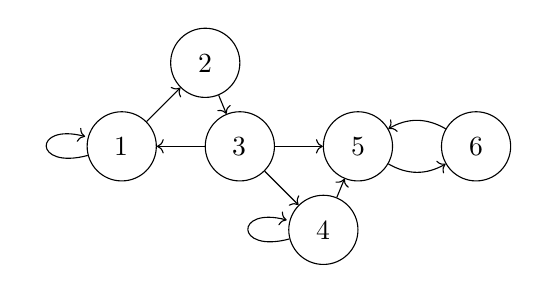
\begin{tikzpicture}[->,auto,node distance=1.5cm]
    \node[state] (1) {\(1\)};
    \node[state,above right of=1] (2) {\(2\)};
    \node[state,right of=1] (3) {\(3\)};
    \node[state,below right of=3] (4) {\(4\)};
    \node[state,right of=3] (5) {\(5\)};
    \node[state,right of=5] (6) {\(6\)};

    \draw
    (1)
    edge[loop left] node{} (1)
    edge[] node{} (2)
    (2)
    edge[] node{} (3)
    (3)
    edge[] node{} (1)
    edge[] node{} (4)
    edge[] node{} (5)
    (4)
    edge[loop left] node{} (4)
    edge[] node{} (5)
    (5)
    edge[bend right] node{} (6)
    (6)
    edge[bend right] node{} (5);
  \end{tikzpicture}
  \end{center}
\end{minipage}
  has communicating classes \(\{1,2,3\}, \{4\},\{5,6\}\), only the last of which is closed.
\end{eg}

\section{Recurrence or Transience}

Introduce notation \(\P_i(\cdot) = \P(\cdot| X_0 = i), \E_i(\cdot) = \E(\cdot|X_0=i)\).

\begin{defi}
The \emph{first-passage time} of \(j\in S\) is
\[
T_j = \min \{n\geq 1: X_n=j\}.
\]
The \emph{first-passage probability} are
\[
f_{i,j}(n) = \P_i(T_j=n).
\]
\end{defi}

\begin{defi}
  \(i\in S\) is \emph{recurrent (or persistent)} if
  \[
\P_i(T_i < \infty) = 1,
  \]
  and \emph{transient} otherwise.
\end{defi}

\begin{thm}
  \(i\) is recurrent if and only if
  \[
    \sum_{n\geq0}^{}p_{i,i}(n) = \infty.
  \]
\end{thm}

Introduce two generating functions
\begin{align*}
  P_{i,j}(s) &= \sum_{n\geq0}^{ }p_{i,j}(n)s^n \\
  F_{i,j}(s) &= \sum_{n\geq0}^{ }f_{i,j}(n)s^n \\
  \delta_{i,j} &= p_{i,j}(0) =
                 \begin{cases}
                   1 & i = j \\
                   0 & i \neq j
                 \end{cases}\\
  f_{i,j}(0) &= 0 \forall i,j
\end{align*}

\appendix

\section{Resources}


Reading list: Probability, an introduction Grimmet, Welsh, 2nd edition, Chapter 12

%webpage: www.statslab.cam.ac.uk/~grg/
\end{document}